\documentclass[12pt,oneside]{report} 
\usepackage[a4paper,width=150mm,top=25mm,bottom=25mm]{geometry}
\linespread{1.5} 
\usepackage{helvet}
\usepackage{graphicx}
\usepackage[font={small,it}]{caption}
\usepackage{tabularx}
\usepackage{adjustbox}
\setcounter{tocdepth}{4}
\setcounter{secnumdepth}{4}
\usepackage[numbers,super,square, compress]{natbib}
\usepackage[euler]{textgreek}
\usepackage[citecolor=blue]{hyperref}
\hypersetup{colorlinks=true, linkcolor=black, urlcolor=blue}
\renewcommand{\familydefault}{\sfdefault}
\title{Chimeric Antigen Receptor T Cells: Current Strategies and Road to Solid Tumour}
\author{Ho Hin Nicholas Wong \\ Supervisor: Professor Andrew Martin \\ BIOC0021: Advanced Investigative Project in Molecular Biosciences \\ University College London}
\date{}
\renewcommand\thesection{\arabic{section}}

\begin{document} 
\maketitle{} 


\chapter*{Acknowledgement}
I would like to express my gratitude to all the advices given by Professor Andrew Martin during this period of time.
\chapter*{Abstract}
Adoptive cell therapy by infusing engineered T cells expressing chimeric antigen receptor (CAR) is one of the uprising and promising approaches by genetically redirecting our own immune cells to target tumour cells. We have seen great success in CAR T cell therapy targeting B lymphocytes leukaemia, but there is still a long road ahead of us to translate the application of CAR T cell therapy from liquid cancer to solid tumours. This review highlights the current understanding and drawbacks of applying CAR T cell therapy in leukaemia and discusses the challenges when targeting solid tumour including (1) trafficking (2) infiltration (3) hostile tumour microenvironment. We also present some possible approaches to tackle the problems in various directions including (1) further modulations in CAR construct design to improve efficacy (2) explore the potential complementation with other therapies. The importance of preclinical models in order to balance the efficacy and safety of the therapy is also discussed.

\tableofcontents

\newpage
\section{Introduction} 
Chemotherapy, radiotherapy and surgery have been the staples in treating cancer over the decades. However, the likelihood of complete remission is close to zero. Despite the advances in immunotherapies including the usage of monoclonal antibodies, immune checkpoint inhibitor and adoptive cell transfer which are more effective and have less side-effects compared to traditional therapies, treatment responses vary greatly among different patients due to tumour heterogeneity. Chimeric Antigen Receptor (CAR) T cell treatment is the new beacon of hope which harnesses the immune system and directs T cells to target tumour associated antigens (TAA) and tumour specific antigens (TSA). These are expressed on the tumour cell surface in which the epitope is usually unique to the cancer type. As early as 1980s, the idea of constructing a chimeric T cell receptor as functional receptors that could bind to specific antigen was first described\citep{first, KUWANA1987960} and tested. The study presented a way to construct and express a genetically modified chimeric T cell receptor consisting the constant domains of the receptor fused with the variable domains originated from an antibody that bind to specific antigen. Recently, two anti-CD19 CAR T-Cell therapies were approved by the FDA in the US, Gilead's Yescarta (Axicabtagene ciloleucel, October 2017) for large B-cell lymphoma and Novartis's Kymriah (Tisagenlecleucel, August 2017) for B cell acute lymphoblastic leukaemia; the approval in the UK was confirmed a year later. NHS struck a deal with Novartis and Gilead, providing Kymriah\citep{Kymriah} and Yescarta\citep{Yescarta} to 200 patients per year. This is a very small number of patients that can benefit from CAR T Cell therapy and clear evidence show that there is huge potential in applying CAR T cell in solid tumours which account for more new cancer cases in the UK\citep{CRUK}. This review will focus on the design of CAR and how modifications in construct can overcome current obstacles that affect the efficacy of the therapy when applied in solid tumours.


\subsection{Design of CAR T Cell}
The first generation of CAR T-Cell therapy consists of only an ectodomain with a single-chain variable fragment (scFv) and a spacer domain, a transmembrane domain and a CD3\textzeta{} endodomain that couples the antigen recognition signal to intracellular signal pathways that activates the T cell\citep{CD3} (Figure 1). The second generation CAR adds in CD28 as the costimulatory molecule that was shown to enhance T cell proliferation, survival \citep{survival} and cytokines production \citep{activation}. Some second generation constructs showed that using CD28/CD3\textzeta{} CAR augments the exhaustion of CAR T cell under persistent CAR signalling \citep{exhaustion} and 4-1BB(CD137)/CD3\textzeta{} CAR as the costimulatory domain showed a better CAR T cell persistence and increase in number of CD8+ central-memory T cells\citep{CD28-1, CD28-2, CD28-3, 4-1BB}. 
\\\\This difference may be explained by the alterations of T cells metabolism when using different costimulatory domains\citep{CD28-2}. CD28/CD3\textzeta{} CAR increases glycolytic metabolism by activating the Akt pathway\citep{CD28-5} which increases uptake of glucose by upregulating gene for glucose transporters. This encourages effector cell differentiation and expansion results in a stronger anti-tumour effect in the early stage. 4-1BB/CD3\textzeta{} CAR increases mitochondrial biogenesis and fatty acid oxidation by switching to metabolic pathway controlled by AMP-activated protein kinase (AMPK) which improves persistence\citep{CD28-2}. A study using gene set enrichment analysis (GSEA) showed that CD28/CD3\textzeta{} CAR showed a higher expression of genes that code for inhibitory receptors (PD1, LAG3, HAVCR2, CTLA4, BTLA and CD244) and also exhaustion-associated transcription factors (TBX21, EOMES, Blimp-1 and IKZF2)\citep{CD28-4-1BB-3}. 4-1BB/CD3\textzeta{} CAR on the other hand showed higher expression of genes that are related to memory T cell differentiation such as KLF6, JUN, JUNB and TNFRSF4 (OX40)\citep{CD28-4-1BB-3}. They also showed a higher expression of CD200\citep{CD28-4-1BB-3} which was shown to suppress memory T cell function when over-expressed on acute myeloid leukaemia (AML) blasts\citep{CD200}. 
\\\\These evidence show that careful consideration of costimulatory domain used in second generation CAR construct is crucial in achieving maximum therapeutic effect. The third generation of CAR consists of two costimulatory domains with CD28 coupled with CD27, CD134 (OX40), 4-1BB \citep{CD137} and ICOS. This further fine-tunes the T cell response as it was shown that CD28/4-1BB CAR T-cell exhibited more cytokines release, increased cytotoxicity and improved survival compared to second generation CAR T-cell but some also showed decreased efficacy\citep{CD28-4-1BB-1, CD28-4-1BB-2}. 
\\\\The fourth generation is known as T cell redirected for universal cytokine killing (TRUCK), which the T cell activation signal induces cytokines production. One particular design is constructed such that the interleukin (Il)-12 expression is put under the control of a NFAT transcription factor response promoter that consists of six NFAT-binding motifs\citep{il12, il122}. There are different ways that Il-12 can help enhance the antitumour ability of CAR T-Cell. It alters the functions of tumour-associated macrophages (TAM) and tumour-infiltrating macrophages, changing their immunosuppressive profile and increase their proinflmmatory activities (producing TNF-\textalpha, Il-15 and Il-18) \citep{il12macro}. This bridges the innate and adaptive immunity as Il-15 is crucial in expansion and maintenance of memory CD8 T cells \citep{il15cd}. Il-18 is known to synergise with other cytokines to increase the proinflmmatory potential of T cells\citep{il18}. Antitumour activity of natural killer T (NKT) cells can be activated by the combined effect of Il-12 and Il-18\citep{NKT}. NKT cells activated by Il-12/Il-18 produce IFN-\textgamma{} or IL-2 can activate NK cells to further augment the antitumour effect\citep{NKT}. Also, Il-12 can direct the development of CD4+ T cells towards Th1 subtype \citep{cd4il12, cd4il122, cd4il123, cd4il124} which promotes the proliferation of cytotoxic CD8+ T cells. The potential of adding different cytokines is still being explored currently.

\begin{figure}[h!]
  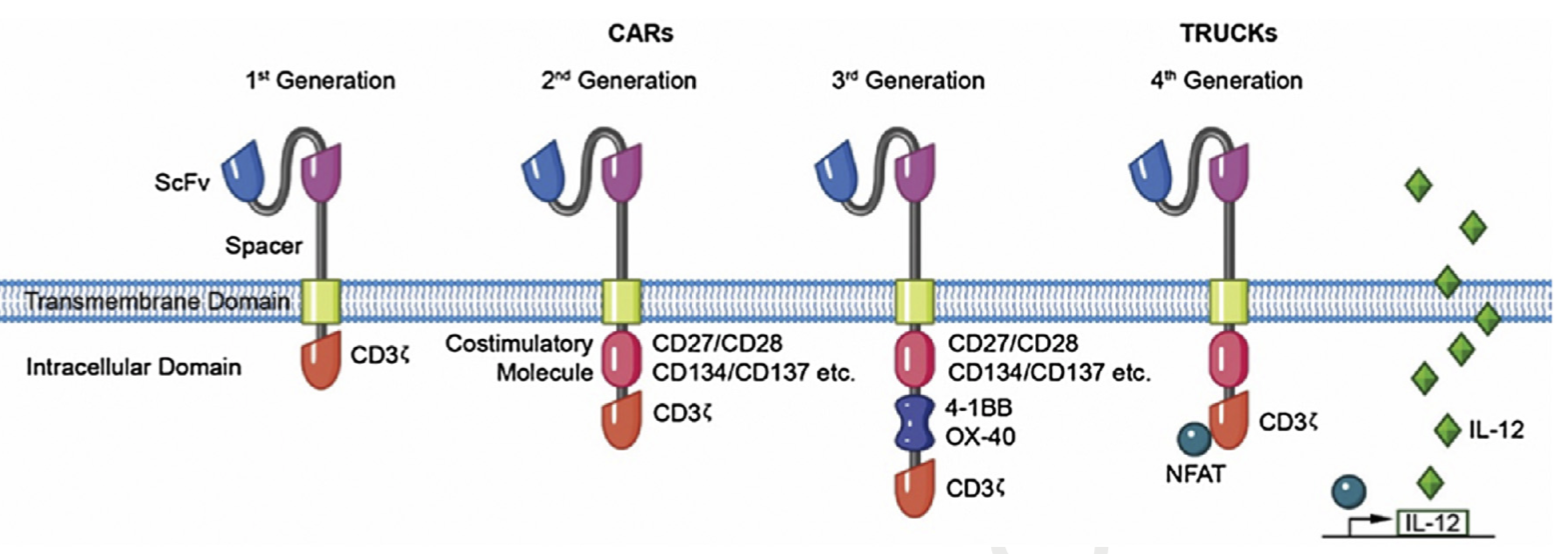
\includegraphics[scale=0.5]{generation.png}
  \caption{Basic strucuture of chimeric antigen receptor (CAR) throughout the generations Taken from: Aaron J.Smith, 2016\citep{fig1}}
\end{figure}
\subsubsection{Spacer Domain} 
The spacer domain links the scFv domain to the intracellular stimulatory domains of the CAR construct. The most commonly used domains are derived from Fc region of IgG1, IgG4 or the extracellular region of CD8\citep{hinge}. The use of IgG4-CH3 derived spacer domain significantly increased the expansion of anti-CD19/mesothelin CAR T cell by about 40\%\citep{hinge} but the use of IgD derived spacer domain anti-MUC1 CAR T cell did not show as much improvement in expansion (about 10\%)\citep{hinge}. This suggests that the origin of the spacer domain and the antigen targeted by the CAR T cell might alter the effectiveness of spacer domain inclusion in the CAR construct. Interestingly, the expansion of CD8+ T cell was less significant than CD4+ T cell when the spacer domain was included\citep{hinge} but if they were isolated and cultured separately they showed no difference in number. The underlying mechanism of spacer domain affecting T cell differentiation is still unclear but it is clear that the expansion of CD4+ T cell requires the prescience of CD8+ T cell. 
\\\\On the other hand, other studies reported that the inclusion of IgG1-CH2-CH3 spacer domain hindered the efficacy of anti-CD19\citep{hinge-2}/CD30\citep{hinge-3} CAR T cell. A hypothesis was made that the inclusion of CH2 domain increases the binding affinity to Fc gamma receptors (Fc\textgamma Rs) as there are two Fc\textgamma R binding motifs within CH2 (233–-236 (ELLG) and N297). This binding results in accidental activation of CAR T cell upon interaction with cells expressing Fc\textgamma Rs such as monocytes and natural killer cells\citep{hinge-3}. Four different spacer domain designs were compared\citep{hinge-7} to evaluate the trafficking and killing potential of the CAR T cell, (1) M1: IgG1-CH2CH3 with mutating ELLG at position 233–-236 to PVA and N297Q mutation (2) M2: IgG2-CH2CH3 with N297Q mutation (3) X2: IgG2 (4) X$_{3}$2: IgG2-CH3. M1 and M2 both showed improved trafficking with M2 being superior in escaping from the lung\citep{hinge-7} where the CAR T cells with original spacer domain design were trapped at. However, they failed to promote tumour regression and it was hypothesised that the expression of CH2CH3 domain promotes cell senescence and favours differentiation towards memory phenotype. The production of X2 CAR T cells which the whole CH2CH3 domain was deleted confirmed the hypothesis as they retained the naive phenotype, however antigen recognition was affected\citep{hinge-7}. Inclusion of CH3 domain (X$_{3}$2) successfully rescued the antitumour activity without inducing cell senescence and they showed superior tumour regression and longest \% survival in mouse model\citep{hinge-7}. 
\\\\Other studies which used IgG4 with mutated CH2 domain (L235E and N297Q) in xenograft model targeting CD19\citep{hinge-4} and Il-13R\textalpha 2\citep{hinge-5} showed similar results with improved CAR T cell trafficking, antitumour activity and persistence. The length of the spacer required was shown to be dependent on the distance between the CAR T cell and target epitope\citep{hinge-6}. These findings highlight the importance of optimising the spacer domain in maximising efficacy of CAR T cell and should be designed on a case-by-case basis. 

\section{Current Understanding}
\subsection{Major Target}
The most studied antigen and the only one used in approved therapies is CD19, a biomarker and target for B lymphocyte malignancies. The use of CAR T-Cells targeting CD19 have shown significant antitumour efficacy and clinical success from 57 up to 90\% overall complete remission rate when treating relapsed/refractory B cell acute lymphoblastic leukaemia (B-ALL) in children and young adults \citep{ALL, ALL2, acute, acute2}, relapsed/refractory chronic lymphocytic leukaemia (CLL)\citep{chronic} and B-cell non-Hodgkin lymphoma (NHL)\citep{lymphoma}. Despite proven effective against B lymphocyte malignancies, there are still potential toxicities that affect the survival rates of patients after the therapy and we need to understand the origin of those toxicities to prevent the potential of similar toxicities when applying CAR T cell therapy in solid tumours.

\subsection{Toxicity}
\subsubsection{Cytokine Release Syndrome (CRS)} 
Second generation constructs of CAR T-cell increase cytokine production and achieve enhanced cytotoxicity but they can be a double-edged sword. The immune activation induces adverse events (AEs) such as hypotension, febrile neutropenia, acute vascular leak syndrome and fevers\citep{cyto-1}. The incorportation of CD28 or 4-1BB expresses differences in cytokines release, 4-1BB induced signalling shows less potency in secreting IFN-\textalpha{} and Il-2 compared with CD28\citep{cyto-9}. It seems that the concentration of cytokine released is correlated with the tumour burden and CAR T cell expansion of the patient\cite{acute2, cyto-2}, indicating that the more effective the therapy is, the higher chance there is developing more severe CRS.  
\\\\In various studies around 10-45\% of patients developed severe CRS (grade $\geq$3 which shows symptoms require and respond to aggressive intervention) \citep{cyto-3, cyto-4, cyto-5, cyto-6, cyto-7, cyto-8}. The most frequently observed cytokines related to CRS are interferon (IFN)-\textgamma, tumour necrosis factor (TNF)-\textalpha, Il-6, Il-10 and Il-2 receptor \textalpha{} (sIL2Ra) (Table1). Currently, CRSs are usually controlled by high-dose steroids such as corticosteroids or monoclonal antibodies (mAb) such as tocilizumab that blocks interleukin receptor, usually Il-6R\citep{ALL}. However, using steroids in CRS management results in depletion of CAR T cells by five-folds when compared with using tocilizumab alone with similar results in reversing CRS symptoms\citep{ALL}. Patients treated with tocilizumab alone showed persisting T cell culture, indicating that tocilizumab did not affect long term T cell survival\citep{chronic} and this suggests that using tocilizumab as the first line of immunosuppressive therapy might be a better choice. It is a tricky situation to balance between the efficacy of the therapy and CRS management, early immunosuppression may result in severe decrease in efficacy but late CRS management can become fatal.  
\begin{table}[!htbp]
\caption{Cytokines related to CRS and their effects on CAR T-Cell therapy clinical trials}
\tiny
\begin{tabularx}{\textwidth}{  p{1.0cm} | p{1.8cm} | X | X }
  \hline			
  Cytokines & Sources & Principle Targets and Functions & Symptoms in CRS \\
  \hline
  \hline
  IFN-\textgamma{} & NK cells, Th1 cells and Cytotoxic T lymphocytes (CTLs) & 
	  {\begin{tabularx}{\linewidth}{X}
	   Macrophages: classical activation \\
	   T cells: Th1 differentiation \\
	   B cells: isotype switching to opsonizing \\
	   Various cells: increases MHC expression and antigen processing to T cells \\
	   \end{tabularx}}
   & Fever, chills, dizziness and headache, fatigue \\
   
  TNF-\textalpha{} & Macrophages, NK cells and T cells &
	  {\begin{tabularx}{\linewidth}{X}
	   Endothelial cells: activation (inflammation) \\
	   Neutrophils and macrophages: stimulates microbicidal activity \\
	   Liver: synthesis of acute phase proteins \\
	   \end{tabularx}}
       &{\begin{tabularx}{\linewidth}{X}
	   Flu-like syndrome, fever, general malaise, rigor, and watery diarrhea, \\
	   vascular leak, inhibits myocardial contractility and vascular muscle tone, \\
	   lung injury, synthesis of acute phase proteins \\
	   \end{tabularx}}\\
 
  Il-2/sIL2Ra & T cells & 
	  {\begin{tabularx}{\linewidth}{X}
	   T cells: proliferation and differentiation into effector and memory T cells \\
	   NK cells: proliferation and differentiation \\
	   B cells: proliferation and antibody synthesis \\
	   \end{tabularx}}
  & Flu-like syndrome, vascular leak, inhibitory actions on myocyte contractility \\
  
  Il-6 & T cells, monocytes, macrophages, fibroblasts and endothelial cells & 
	  {\begin{tabularx}{\linewidth}{X}
	   Augment immune response \\
	   B cells: proliferation of antibody-producing cells \\
	   Neutrophils: stimulates production from the bone marrow \\
	   Liver: synthesis of acute phase proteins \\
	   \end{tabularx}}
  & Fever, chills, nausea, vomiting and fatigue, vascular leak, lung injury \\
  
  Il-10 & Th2 cells and macrophages & 
	  {\begin{tabularx}{\linewidth}{X}
	   Macrophages and DCs: inhibition of the expression of IL-12, costimulators and class II MHC \\
	   \end{tabularx}}
  & Fever, headache, back pain, dizziness \\
  
  Il-12 & Macrophages and DCs & 
	  {\begin{tabularx}{\linewidth}{X}
	   T cells: Th1 differentiation \\
	   NK cells and T cells: IFN-\textgamma{} synthesis, increasing cytotoxicity \\
	   \end{tabularx}}
  & Fever, chills, nausea/vomiting, hypotension, anorexia, myalgia, fatigue, liver toxicity \\
 
  \hline 
\end{tabularx}
\caption*{Cytokine release syndrome observed in CAR T-Cell Therapy\\ Adapted from: Xiao-JunXu 2014\citep{cyto-9}}
\end{table}
\\\\A study suggested that more investigations should be done regarding CRS to isolate cytokines that are required for increasing efficacy of the CAR T-Cell therapy and those that induce adverse events\citep{cyto-8}. Il-6 was chosen as a target due to its excess secretion in CRS and its insignificant role in antitumour activity. This allows us to target CRS-indusing cytokines and apply mAb to reduce toxicity. Il-10 is a potential target that should be studied. It demonstrates both anti- and pro-inflammatory properties which may exert various effects on the efficacy of CAR T cell. It was shown to inhibits the production of pro-inflammatory cytokines by immune cells such as macrophages and Th1 cells during pathogens infection\citep{il10} but was also shown to maintain the function of CD8+ cytotoxic T cells\citep{il10-2}. This dual-role played by Il-10 during inflammation response raises questions about whether inhibiting Il-10 would dampen the antitumour activity of CAR T cell or enhance the activity of other immune cells which may increase the efficacy of the treatment.

\subsubsection{Neurotoxicity} 
There is evidence that early CRS developed after CAR T Cell infusion leads to a higher risk of developing reversible neurological toxicities including confusion, seizure, headache, decreased level of consciousness and in extreme cases death\citep{ALL, cyto-10, cyto-11}. 133 adults with refractory B-ALL, NHL, or CLL applied anti-CD19 CAR T-Cell therapy with 4-1BB as the costimulatory domain after receiving lymphodepletion chemotherapy were studied and 40\% (53/133) of them developed one or more grade $\geq$1 neurological AEs\citep{cyto-11} within 28 days after the infusion. 48 out of those 53 patients with AEs also had CRS. Patients who showed symptoms of CRS such as fever at the earlier stage of the treatment developed a higher grade of neurotoxicity ($\geq$3) compared to those who did not, showing the correlation between CRS severity and the onset and severity of neurotoxicity. 
\\\\The severity of neurotoxicity correlates with the level of C-reactive protein (CRP, acute-phase protein released by the liver responding to Il-6), ferritin and other cytokines (Il-6, IFN-\textgamma{} and TNF-\textalpha) that lead to endothelial activation\citep{ALL, cyto-11}. Real-time monitoring of serum Il-6 level before onset of toxicities is difficult due to time constraint so CRP was chosen and tested as a reporter protein of CRS\citep{ALL}. It was proven successfully that CRP is an excellent indication for CRS as they showed a very strong correlation\citep{ALL}. The combined observations suggest that patients with early fevers and a CRP level reaching certain threshold should be managed as if they have CRS as these indicate a very high risk in developing neurotoxicity. 
\\\\The pathogenesis of neurotoxicity is still unclear, but clinical evidence such as endothelial dysfunction (vascular instability, capillary leakage, disseminated intravascular coagulation) was accompanied with elevation of serum cytokines levels in particular Il-6, IFN-\textgamma{} and TNF-\textalpha{} in patients with severe neurotoxicity\citep{cyto-11}. The study hypothesised that one of the potential causes of neurotoxicity is the vascular leakage of high concentrations of cytokines into the cerebrospinal fluid (CSF) due to disruption of the blood brain barrier (BBB). The permeability of the BBB increased after lymphodepletion chemotherapy, showing higher concentration of protein and leukocyte detected in CSF compared to before lymphodepletion\citep{cyto-11}. This disruption of BBB is considered to be induced by the effects of cytokines\citep{BBB-1}. Although there were some previous arguments regarding the effects of TNF-\textalpha{} on the permeability of BBB\citep{BBB-4}, it was hypothesised to increase the BBB permeability in different ways such as affecting the architecture, increasing the expression of adhesion molecules for immune cells\citep{BBB-5}. BBB-endothelial cells (BBB-ECs) express tight junction (TJ) and adherens junction (AJ) proteins that limit cellular permeability\citep{BBB-1}. TNF-\textalpha{} was shown in a mouse model to downregulate occludin expression in BBB-ECs, which is one of the major components of TJ proteins\citep{BBB-2}. This effect was not observed in any human model, but \textit{in vitro} TNF‐-\textalpha{} and IFN‐-\textgamma{} stimulation were shown to change the architecture of junction proteins without affecting their expression\cite{BBB-2, BBB-3}, however the exact effect of this modulation on the permeability of BBB was not validated. Adhesion molecules such as CXCL10, CXCL9, CX3CL1, CCL3, CCL4 and CCL5 were shown to be upregulated by the combination of IFN-\textgamma{} and TNF-\textalpha{} \citep{BBB-1} and they could induce the chemotaxis of various immune cells towards BBB\citep{BBB-1}. 
\\\\These findings confirm that the patients with more severe CRS have a higher risk of developing neurotoxicity. The increase in BBB permeability leads to cytokines diffusing into CSF and a possible increase in local cytokine production due to migration of immune cells across the BBB. This side effect raises the question of how did the T cell with this CAR construct actually penetrate the BBB. Penetration of the BBB in treating glioma has been a huge problem, therefore a thorough understanding of the molecular basis behind this mechanism is needed.

\subsubsection{Anaphylaxis} 
Sometimes donour-derived T cells are used in the CAR T cell therapy and it is expected to show some degree of graft-versus-host disease (GVHD) which the immune cells in the donor (infused CAR T cells in this case) attack the patient's body's cells. In some cases reversible GVHD symtoms (aggravated hyperbilirubinemia, elevated amino-transferases and chronically aggravated skin damage) were observed \citep{allo-3} but no large number of adverse events had been recorded. In a clinical trial 1 patient out of 4 developed acute anaphylaxis (allergic reaction) which resulted in a lethal cardiac arrest event after the third infusion of anti-mesothelin CAR T cells with 4-1BB stimulatory domain\citep{allo-4}. Given that the same batch of CAR T cells was used in those 3 infusions, it was proposed that the serious adverse event was caused by an accumulated immune response from multiple infusions\citep{allo-4}. Further investigation was conducted based on the suspicion that this adverse event was caused by Ig-E mediated degranulation of mast cells leading to anaphylaxis. Tryptase, which is a marker for mast cells degranulation was recorded to have an elevated level\citep{allo-4}, confirming the adverse event was caused by Ig-E mediated anaphylaxis. The research group suggested future trials that require multiple infusions should be designed such that infusions must not be separated for more than 10 days and all infusions should be completed within 21 days to minimise the chance of class switching from IgG to IgE\citep{allo-4} which causes the mast cell degranulation that leads to anaphylaxis. 
\\\\Interestingly, CD28/CD3\textzeta{} CAR seems to reduce the probability of developing GVHD and increases survival rates when compared to 4-1BB/CD3\textzeta{} CAR or not having a costimulatory domain\citep{allo-5}. The research group hypothesised the repetitive stimulation signals from CAR and alloreactive TCR lead to T cell exhaustion and eventually being deleted, reducing the number of alloreactive CAR T cells\citep{allo-5}. The expansion of CD8+ effector-memory T cells and cytokines production (Il-6, IFN-\textgamma{} and TNF-\textalpha) were significantly impaired when using CD28\citep{allo-5}. This confirmed their hypothesis that T cell exhaustion protects patients from GVHD. This finding also agrees with previous researches that the use of CD28 instead of 4-1BB induces T cell exhaustion and affects the persistence of CAR T cells\citep{CD28-2, CD28-3, CD28-4} and further complicates the balance between proliferation and persistence potential of CAR T cells when choosing different costimulatory domains. This anaphylaxis incident showed that there is a need in setting up a clinical protocol that provides guideline on multiple infusions of CAR T cell. 

\subsubsection{On-Target/Off-Tumour}
The major on-target/off-tumour toxicity observed when applying CAR T cells in leukaemia is B cell aplasia, the depletion of nonmalignant B cells. This is an expected side effect as CD19 is expressed on both malignant B cells and normal B cells so the CAR T cells targeting CD19 will also attack normal B cells. This suggests that B cell aplasia can also be served as an indicator for the effectiveness of the therapy as it correlates with the persistence of CAR T cells in the patient. The severity of B cell aplasia varies from a few months\citep{ALL2, aplasia} to over 15 months\citep{aplasia-3} and CAR T cells using 4-1BB showed a prolonged B cell aplasia\citep{aplasia-2, aplasia-3}, agreeing with the findings that 4-1BB improves CAR T cell persistence. This can be easily managed with infusion of \textgamma -immunoglobulin (IgG) as replacement therapy\citep{ALL2, aplasia-4, aplasia-5} to reduce the risk of infection but the cost of the therapy will be further increased and there is also risk of allergic reaction.

\section{Future CAR development}
Although we have seen great success in applying CAR T Cell therapy in B cell malignancies, there are way more cancer incidences in solid tumours than leukaemia\citep{CRUK} and the next step is to explore the therapeutic potential of CAR T Cell therapy in solid tumours. To translate this technology from liquid to solid tumours, the balance between therapeutic effectiveness and potential toxicities must be evaluated carefully. Targeting solid tumour is more challenging than leukaemia, as one of the key factors to an effective and safe therapy is unique targetable antigens. CD19 is an excellent target in leukaemia due to its exclusive expression on B cells, even though nonmalignant B cells will also be depleted during the therapy, aplasia can be easily managed. On the other hand, a lot of antigens expressed on cancer cells in solid tumours are also expressed on normal cells and the on-target/off-tumour effect may results in organ damage. Some new CAR designs have been incorporating a suicide gene or a safety switch\citep{blueprints} to produce a more controllable CAR T cell design. Despite the success in treating B cell leukaemia, there are still other hurdles that we have to overcome in order for CAR T Cell therapy to be viable in treating solid tumours.

\subsection{Challenges in Designing CAR T-Cell for Solid Tumours}
\subsubsection{Trafficking} 
CAR T cell localisation to the target tumour site is essential in targeting solid tumours. The expression of E-, P-selectin ligands and L-selectin on the CAR T cells and cell adhesion molecules on the endothelial cells is needed for T cells to roll (slow down during extravasation) on the tumour cells\citep{traffick-2}. Matching between chemokine receptors on CAR T cells and the chemokines released by the tumour cells is also vital in T cell trafficking\citep{traffick-1}. 
\\\\Glioblastoma is the most aggressive brain tumour with high death rates so it will be used to discuss about the importance of adhesion molecules. Activated leukocyte cell adhesion molecule (ALCAM) has a major role in T cell recruitment associated with inflammatory brain diseases\citep{homing}. It has been shown that brain cancer endothelial cells overexpressed ALCAM but they downregulated the expression of intercellular adhesion molecule-1 (ICAM1) and showed no expression of vascular cell adhesion molecule-1 (VCAM1)\citep{homing}. Similar changes were observed in multiple sclerosis (MS) which ICAM1 and VCAM1 act as the secondary signals required to reach the threshold needed to recruit T cells from the bloodstream\citep{MS}. This alteration allows the tumour cells to evade the immune system as T cells cannot adhere to the tumour cells. It is still unclear the effects of the overexpression of ALCAM apart from tumour invasion but ALCAM alone is not sufficient for T cells homing to the tumour cells\citep{homing}. The research group hypothesised that they can apply what they learnt from MS and overcome this immune-evasion mechanism of glioblastoma. An \textit{in vitro} BBB model was created by sandwiching a polycarbonate membrane between primary tumour endothelial cells and pericytes, infiltration ability of CAR T cell was tested with this model.
\\\\In MS, ALCAM colocalises with CD6, which is expressed on activated T cells during T cell migration across the BBB. Poor transendothelial migration of T cells was observed despite the overexpression of ALCAM on tumour endothelial cells\citep{homing}. Therefore the lack of migration was thought to be the result of downregulation of CD6 and a homing system (HS) was developed by re-engineering CD6 on T cells. The prototype HS molecule included a D3 (extracellular domain 3 of CD6) exodomain, an IgG hinge and a CD6 transmembrane and signalling domain. Variants such as multimerising of the D3 domain (denoted as 3HS and 5HS, Figure 2) and some without the signalling domain (HS\textDelta, 3HS\textDelta, 5HS\textDelta) were created to study the effect of crosslinking avidity to ALCAM and importance of CD6 signalling respectively. 
\begin{figure}[h!]
  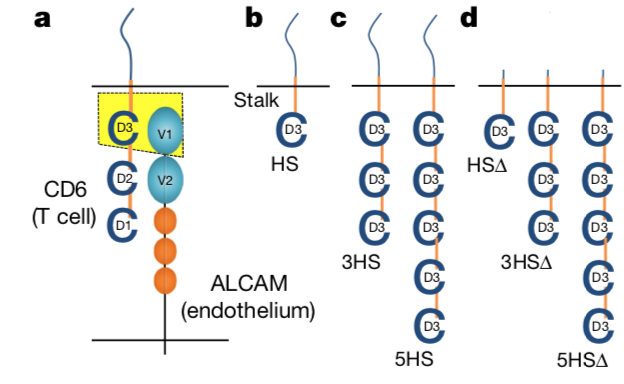
\includegraphics[scale=0.8]{homing.png}
  \caption{Schematic representation of the homing system (a) ALCAM binding to CD6 (b) prototype HS (c) multimerisation of D3 domain (d) without signalling domain \\ Taken from: Heba Samaha 2018\citep{homing}}
\end{figure} \\
T cells with a HS showed more frequent capturing, rolled more slowly and stopped more quickly when they were in contact with ALCAM+ cells compared to normal T cells. They were also more resistant to mechanical detachment which allows them to be less affected by the fluctuating blood flow common in the tumour neovasculature which is chaotically arranged with blind ends. The next step is incorporate this HS design into CAR T cell and validate its effectiveness in clinical trials.
\\\\\textit{In vivo} migration assay had shown that the matching of chemokine receptors expressed on T cells and the chemokines released by the tumour cells is also essential in T cell trafficking\citep{CCR2-2, CCR, CCR-2}. Normal T cells activated by anti-CD3/anti-CD28 beads via the T cell receptor upregulated the expression of chemokine receptor CCR5, CCR7 and CXCR3 were shown to be attracted to tumour cells releasing the respective chemokines\citep{CCR2}. They found very little concentration of these chemokines in patients with malignant mesothelioma but instead CCL2 was highly secreted\citep{CCR2}. However, the chemokine receptor CCR2b was poorly expressed on the anti-mesothelin CAR T cells they were using, so modification was done by transducing CCR2b into the CAR construct\citep{CCR2}. There was a significant increase in infiltrated T cells\citep{CCR2} ($>$12.5 fold) and augmented antitumour activity as well with CAR$+$CCR2b T cells when compared to CAR T cells without the CCR2b\citep{CCR2} (killing ~20$\%$ more tumour cells). The increased infiltration and augmented antitumour activity should be interpreted as the result of enhanced trafficking (more CAR T cells were accumulated at the tumour site) as there were no other changes to the construct that could affect the efficacy of the CAR T cell except an improved chemotaxis ability. Similar results were obtained by another research group when transducing CCR2b to anti-GD2 CAR T cells targeting neuroblastoma\citep{CCR2-2} showing a $>$10 fold increase in trafficking and enhanced killing capacity. Despite different CAR constructs were used (second generation 4-1BB in anti-mesothelin CAR and third generation CD28/OX40 in anti-GD2), the CAR T cells with coexpression of CCR2b-CAR showed enhanced killing. 
\\\\This suggests that the incorporation of chemokine receptor in the CAR construct matching the chemokine released by the tumour and a homing system might be a way to further improve antitumour efficiency by enhancing the trafficking of CAR T cell. There has not been any study that evaluate the combined effect of applying both approaches and more experimental data is needed.
\subsubsection{Infiltration} 
Another major challenge we need to overcome is the penetration of the physical barrier surrounding solid tumours. Tumour stromal environment which is common in solid tumours consists of cancer-associated fibroblasts (CAFs), immune cells, endothelial cells, pericytes and an extracellular matrix (ECM) composed of collagen, elastin, fibrilin and proteoglycans\citep{heparanase}. In order to reach the tumour cells, T cells must be able to degrade the ECM components. 
\\\\Heparanase (HPSE), the enzyme that can cleave the heparan sulphate chains of the heparan sulphate proteoglycan (HSPG) was shown to be downregulated in \textit{in vitro} expanded T cells\citep{heparanase}. The study investigated the invasiveness of 4 groups of T cells which they categorised as (1) freshly isolated resting T cells (FI-T cells) (2) briefly activated T cells (BA-T cells) (3) T cells activated for 24 hours (4) long-term \textit{ex vivo}-expanded T cells (LTE-T cells, 12-14 days)\citep{heparanase}. BA-T cells demonstrated the most effective invasion of the ECM (34\% $\pm$ 8\%) when compared to both FI-T cells (23\% $\pm$ 8\%) and LTE-T cells (8\% $\pm$ 6\%)\citep{heparanase}. This observation was explained by the downregulation of \textit{HPSE} mRNA after T cell activation but the molecular basis of this change was not known. The authors suggested this change was due to the accumulation of full-length p53 which binds to the promoter of the \textit{HSPE} gene and block the transcription but more experimental data is needed to support this hypothesis. They showed that the coexpression of CAR and heparanase in LTE-T cells rescued their tumour infiltration and antitumour capacity in xenograft models\citep{heparanase} and further clinical trials should be carried out. 
\\\\The matrix metalloproteinases (MMPs) enzyme family has been considered to be an essential regulator in tumourigenesis and cancer progression due to their tissue remodelling nature. MMP-2 and MMP-9 were shown to be associated with solid tumours progression such as breast and brain cancer\citep{MMP2, MMP2-2, MMP9}. Other MMPs (MMP-2, -3, -9, -13, -14) had been shown to contribute to epithelial-mesenchymal transition which epithelial cells lose their cell-cell adhesion and increase their cell migration ability, leading to metastasis\citep{MMPs}. 
\\\\Interestingly, MMP-8 has shown a protective role in in tongue and breast cancer as a metastasis suppressor in recent studies and the overexpression of MMP-8 positively correlated with the survival rate of patients\citep{MMP8, MMP8-2, MMP8-3}. Tumour cells expressing MMP-8 showed reduced invasive capacity and increased cell adhesion\citep{MMP8-4}. However, MMP-8 expression is also associated with the progression of certain cancers such as ovarian\citep{MMP8-5} and liver cancer\citep{MMP8-6}. The protective nature of MMP-8 was first discovered 10 years ago\citep{MMP8, MMP8-2} but the mechanism was not understood then. The research demonstrated the expression of MMP-8 in breast cancer cells reduced their migration and invasion ability\citep{MMP8-8}. Further investigation showed that MMP-8 cleaves decorin\citep{MMP8-8}, a matrix protein and activated decorin prevents the activation of TGF-\textbeta{} 1 by binding to it. Reduced availability of TGF-\textbeta{} 1 leads to reduced miRNA-21 level\citep{MMP8-8} which usually inhibits expression of tumour suppressor protein programmed cell death 4 (PDCD4). Overexpression of miRNA-21 was shown to be sufficient in reverting the antimetastatic effect of MMP-8\citep{MMP8-8}, supporting the finding that MMP-8 exerts its effects through miRNA-21. Due to these pivotal roles MMP-8 plays in different cancer types and stages\citep{MMP8-7}, it is clear that we should explore the potential of using MMP-8 in new therapeutic approach. Given that overexpression of MMP-8 hinders the migration and invasiveness of tumour cells, perhaps MMP-8 knockout in the CAR T cell can improve the trafficking to the tumour site and infiltration of solid tumour. 
\\\\These findings suggest that incorporating the gene for enzymes that can break down the ECM and potential MMP-8 knockout in the CAR construct can enhance the efficacy of CAR T-cell therapy targeting stroma-rich solid tumours by equipping them with enhanced infiltration ability.
\subsubsection{Microenvironment} 
The solid tumour microenvironment (TME) has been proven to be hostile to T cell due to its metabolic landscape and immunosuppressive nature. When tumour grows in size it requires more oxygen and nutrients supply. Tumour cells release vascular endothelial growth factor (VEGF) which induces angiogenesis, the formation of new blood vessels\citep{VEGF}. However, these newly formed blood vessels are usually poorly organised and also have a lot of blind ends resulting in local hypoxia (low oxygen concentration) area within the tumour\citep{hypoxia}. Genes are upregulated by hypoxia-inducible factor (HIF-1) as the \textalpha{} subunit of HIF is less degraded via the ubiquitin-proteasome system and can translocate into the nucleus and binds to the \textbeta{} subunit to be fully functional.
\\\\Hypoxia has been shown to increase the expression of programmed cell death ligand-1 (PD-L1) in a HIF-1\textalpha -dependent manner which leads to increased apoptosis of T cells, thus avoiding the immune system from targeting the cancer cells\citep{hypoxia-9}. PD-L1 mRNA and protein expression level were upregulated under hypoxic conditions and HIF-1\textalpha{} knockdown experiment indicated that there was a correlation between HIF-1\textalpha{} level and \textit{PD-L1} gene expression level\citep{hypoxia-9}. Chromatin immunoprecipitation (ChIP) assay confirmed that HIF-1\textalpha{} interacted with the \textit{PD-L1} gene and blocking either PD-L1 or PD-1 using antibodies eradicated the T cells-mediated cell lysis resistance of tumour cells\citep{hypoxia-9}. PD-1 and cytotoxic T-lymphocyte–-associated antigen 4 (CTLA-4), which belong to the inhibitory CD28 receptors family are upregulated in activated T cells and their interaction with their ligands (PD-L1/2 expressed on tumour cells and CD80/86 on antigen presenting cells) send an inhibitory signal that prevent the expansion of activated T cells\cite{PD-1}. They reprogramme the T cell metabolism with different pathway where PD-1 promotes fatty-acid oxidation by upregulating the rate-limiting enzyme of FAO and CTLA-4 inhibits glycolysis by inhibiting expression of glucose transporters without promoting FAO\cite{PD-1}. This shift in metabolism inhibits the differentiation of T cell into effector phenotype and restricts their antitumour activity. PD-1 blockade\citep{block} and knockout\citep{knockout} complementing CAR T cell therapy have shown some success with improved efficacy in a case specific manner with no CRS and other adverse events observed, suggesting that immune checkpoint inhibition is useful in augmenting CAR T cell therapy effectiveness and reduce the toxicity when targeting solid tumours. However, the correlation between using immune checkpoint inhibition and reduced toxicity is still unclear and the molecular basis should be studied.
\\\\Also, HIF-1\textalpha{} contributes to the glycolytic metabolism shift by upregulating enzymes required in glycolysis such as hexokinases, phosphofructokinase 1 and phosphoglycerate kinase 1\citep{hypoxia-3}. Glucose uptake is increased by the upregulation of glucose transporters, GLUT1 and GLUT3\citep{hypoxia-4} which further favours this shift in metabolic pathway. The low oxygen concentration and depletion of glucose in the hypoxic area of the tumour inhibits the proliferation of T cell\citep{CD28-5, hypoxia-5}, explaining the inefficient killing ability of T cells in the TME. There are mixed reviews on the effects of HIF-1\textalpha{} on T cell and the therapeutic outcome. CD8+ cytotoxic T lymphocyte(CTL)-mediated cell lysis was impaired when tumour cells overexpress HIF-1\textalpha{} under hypoxic conditions\citep{hypoxia-6}. On the other hand, elevated HIF-1\textalpha{} level in von-Hippel Lindau tumour suppressor(VHL, inhibitor of HIF by targeting it for ubiquitylation and proteasomal degradation)-deficient CTL\citep{hypoxia-7} resulted in improved cytotoxicity. These observations indicate that HIF-1\textalpha{} has varied effects on T cell proliferation and cytotoxicity in the TME. \\\\
\textbf{Oxygen Sensitive CAR} \\
Oxygen-sensitive subdomains of HIF-1\textalpha{} have been incorporated in CAR design in recent study to produce a CAR T cell that can sense the oxygen level and express the CAR in hypoxic conditions\cite{hypoxia-8}. Three constructs were design by fusing various domains with the CAR that contain known proline residues (P402 and P564) which are hydroxylated to be targeted by VHL. The constructs with a large HIF-1\textalpha{} domain (amino acid 380--603, HIF-CAR1, Figure 3) and N-terminal domain (amino acid 344--417, HIF-CAR2, Figure 3) successfully demonstrated that under hypoxic conditions, surface expression of CAR were significantly increased (about 50\% increase) compared to normoxic conditions\cite{hypoxia-8}. The third construct with the C-terminal domain (amino acid 530--652, HIF-CAR3, Figure 3) did not show similar effect. This suggests that P402 which was included in HIF-CAR1/2 is more important in oxygen sensing. They also showed promising safety as the cell surface expression of HIF-CAR1/2 reduced when incubated under normoxic conditions after the previous experiment\cite{hypoxia-8}. This indicates that they were actually oxygen-sensitive and there is little risk in on-target/off-tumour toxicity and should be considered a essential part of the CAR construct as hypoxia is a very common indication of solid tumours. 
\begin{figure}[h!]
  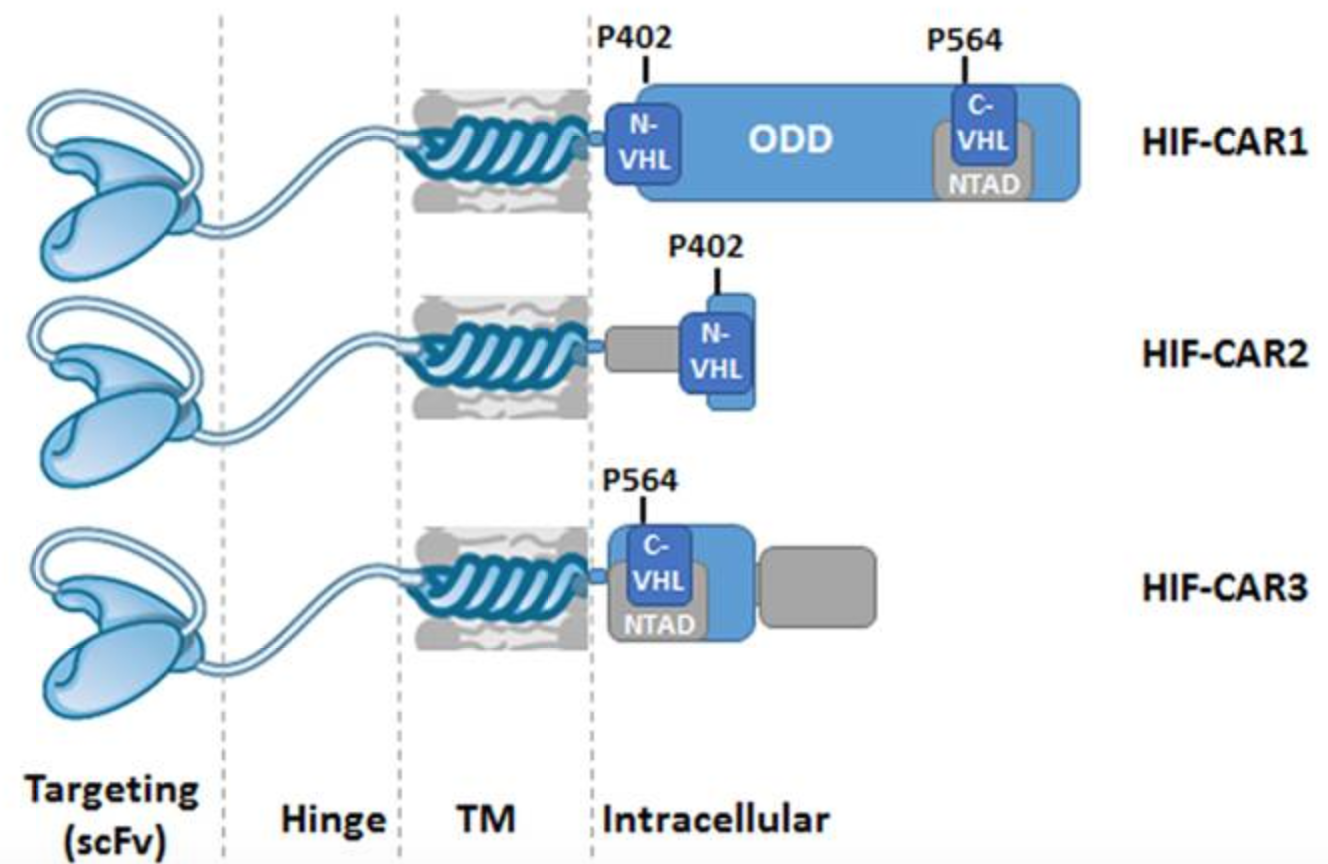
\includegraphics[scale=0.35]{HIF-CAR.png}
  \caption{Schemetic representation of oxygen-sensitive CAR design, ODD: Oxygen-Dependent Degradation domain \\
   Adapted from Alexandre Juillerat, 2017\citep{hypoxia-8}}
\end{figure} \\\\\\
\textbf{Regulatory T cell} \\
Regulatory T cell (Treg) is a subset of T cells that maintains immune tolerance to self-antigens so they are considered immunosuppressive. They downregulate the proliferation of T cells via chemokines such as TGF-\textbeta, Il-10 and Il-35\citep{Treg}. In the tumour microenvironment, tumour-infiltrated dendritic cells (DC) were shown to release chemokines such as CCL22\citep{Treg-2, Treg-3}, CCL17\citep{Treg-2}, CCL28\citep{Treg-4}, CCL5\citep{Treg-5} and CXCL1\citep{Treg-6} that recruit Treg in \textit{in vitro set-up\citep{Treg-2, Treg-3, Treg-4}} and various cancers\citep{Treg-3, Treg-4, Treg-5, Treg-6}. Treg can exert its inhibitory functions by producing adenosine and prostaglandin E2 (PGE2) which affect the adenosinergic pathway via cAMP signalling\citep{Treg-7, Treg-8}. They mediate immune suppression in a similar fashion by ligating to their G protein-coupled receptor (A2AR/A2BR and EP2R/EP4R respectively) expressed on the immune cells\citep{Treg-7, Treg-8}. This signal increases expression of adenylate cyclase (AC) thus cAMP concentration. cAMP then activates its downstream signalling molecule protein kinase A (PKA) which can transduce either proapoptotic or antiapoptotic signal by altering genes transcription\citep{cAMP}, there were evidence that this signalling pathway is proapoptotic in T cells\citep{cAMP-2, cAMP-3, cAMP-4}. A "two hit" approach of direct killing the tumour cells and rescuing the immune response due to the inhibition of this cAMP-PKA pathway was suggested\citep{cAMP-5} (Figure 4). \\
\begin{figure}[h!]
  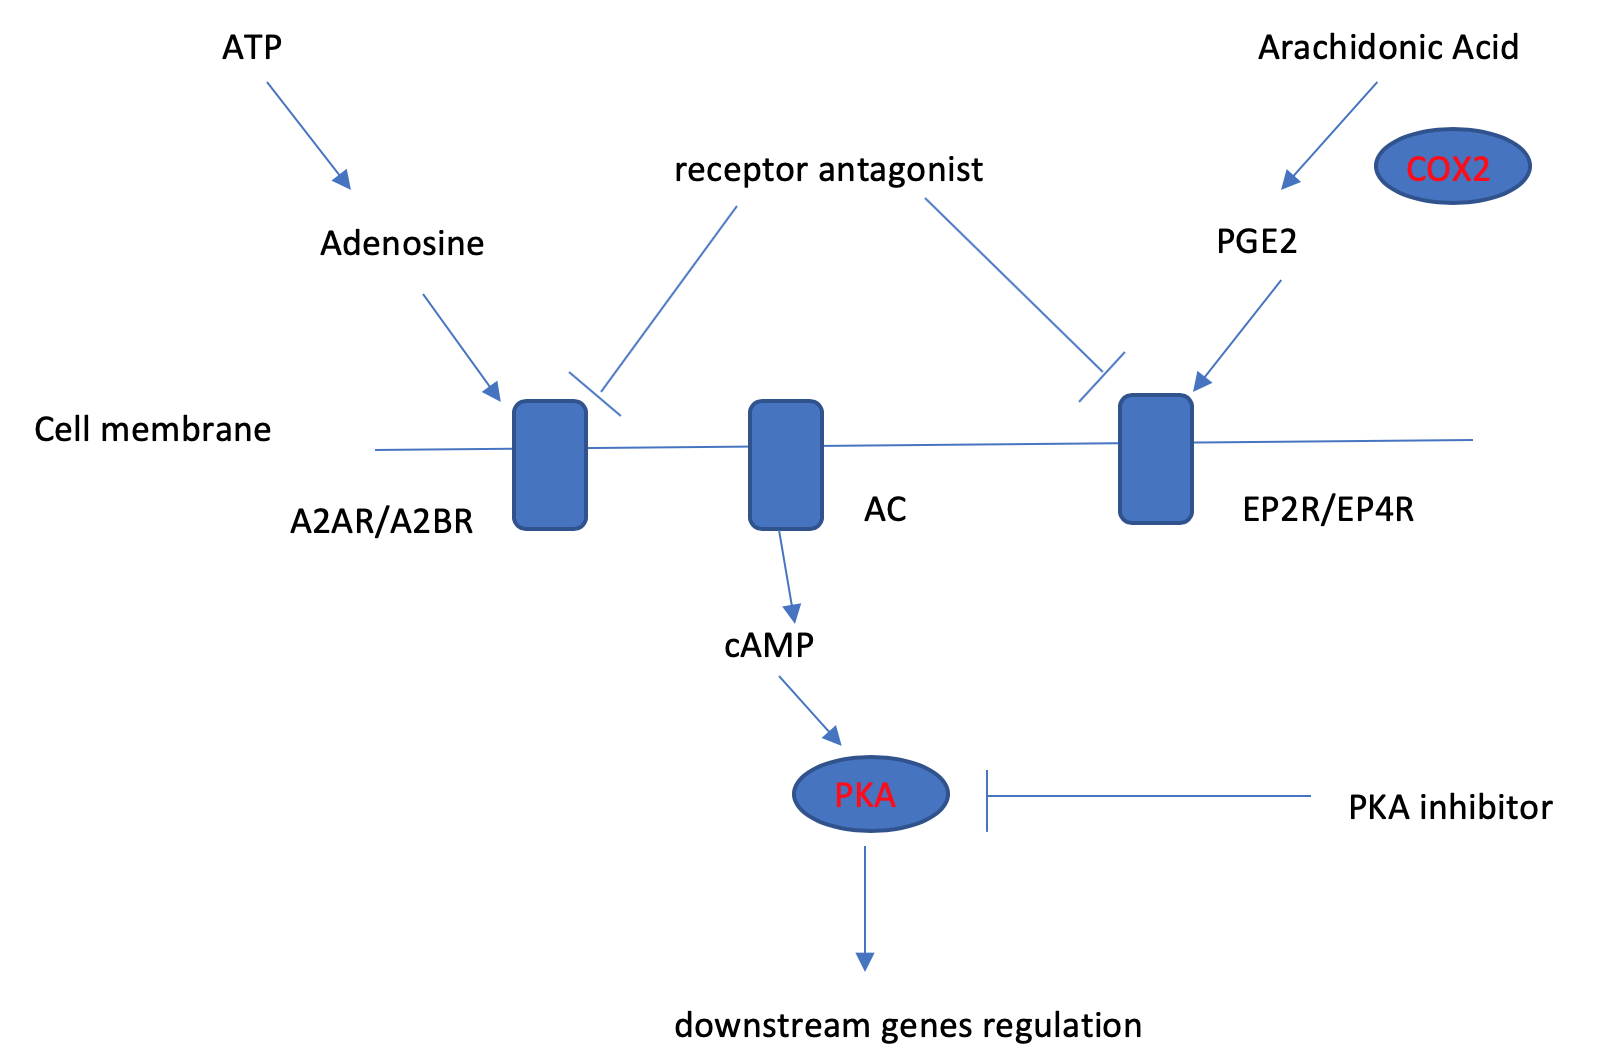
\includegraphics[scale=0.35]{PKA-2.png}
  \caption{The PKA pathway in the "two hit" therapeutic approach schematic}
\end{figure}
\\\\There are multiple targets in this pathway that we can modulate (Figure 4) and it has been shown that disrupting PKA localisation improved CAR T cell trafficking and antitumour activity in mouse models\citep{cAMP-6}. PKA needs to be in close proximity to adenylate cyclase by anchoring to the cell membrane via A-kinase anchoring proteins (AKAP) and ezrin is one of the most studied members\citep{ezrin}. A peptide named regulatory subunit I anchoring disruptor (RIAD) was designed and a region of gene upstream of the PKA binding domain of ezrin named RI specifier region (RISR) was discovered to enhance binding of RIAD to PKA in previous study\citep{ezrin-2}. The research group hypothesised that the inclusion of RISR-RIAD transgene into the CAR construct can improve the efficacy by disrupting the localisation of PKA towards the cell membrane. The CAR T cells with the transgene showed resistance to adenosine and PGE2, antitumour activity was greatly improved with 40--50\% reduction in tumour volume\citep{cAMP-6}. One unexpected observation from the experiment was the increase in number of CD8+ and CD4+ T cells with CD8+ being more dominant. PKA phosphorylates phosphorylase kinase and keeps it in its active form which phosphorylates glycogen phosphorylase, which then promotes the breakdown of glycogen to glucose\citep{PKA}. The inhibition of cAMP-PKA pathway should have reduced the supply of glucose which is vital in the glycolytic metabolism that favours the expansion of T cell, suggesting there might be other effects when disrupting the cAMP-PKA pathway that alters the T cell behaviours. 
\\\\Although this attempt successfully improved the efficacy of CAR T cell therapy, it was done in mouse model which might not have the same tumour microenvironment as human. Also different tumour types might not react in the same way when the cAMP-PKA pathway is disrupted but it demonstrated that the immunosuppressive signals from Treg could be disrupted thus restoring the function of CAR T cell. 

\subsection{Additional Tools}
Due to tumour heterogeneity, every tumour is unique and they respond to treatments differently\citep{heterogeneity}. Intratumour heterogeneity originate from subclonal expansion of some tumour cells with gain of function mutations as a result of genome instability. This leads to failure of therapy and high chance of relapse when some of the tumour cells survive\citep{heterogeneity}. Plotting a phylogenetic tree of the tumour using bioinformatics tools can allow us to distinguish between clonal and subclonal mutations\citep{heterogeneity} and identify driver genes/mutations that influence and contribute to tumour progression\citep{CATH}. 
\subsubsection{Safety/Efficacy Monitoring: Organoid}
We discussed in the previous sections about the importance of balance between efficacy and safety. The identification of driver genes/mutations can help us to design CAR with a scFv that target a more uniquely mutated protein expressed on the surface of the tumour cells and increase the efficacy of the therapy. There have not been as many adverse events reported in treating solid tumours with CAR T cell compared to targeting leukaemia but there are still various levels of CRS\citep{CRS-2, CRS-3}, on-target/off-tumour\citep{on-target} toxicity and even fatal cases\citep{allo-4, fatal} reported in clinical trials. These adverse events show that we require a reliable system to assess the potential risks before applying the CAR T cell to the patients, assessment of effectiveness of the CAR T cell with a preclinical model is essential to maximise the benefit of the therapy.
\\\\To test the effectiveness of antitumour therapy, 3D models that could probe the \textit{in vivo} interactions of the tumour and its surrounding were developed\citep{organoid}. An air-liquid interface (ALI) method propagated patient-derived organoid (PDO) was developed which could imitate the tumour microenvironment (TME)\citep{organoid} and allow us to test the CAR T cells. The research group successfully constructed PODs from 100 patients with 28 unique cancer subtypes and they all preserved the tumour stroma architecture with the tumour infiltrating immune cells population also presented\citep{organoid} (CD4+ and CD8+ T cells, CD3+ T cells with PD-1 expression, B cells, natural killer cells, natural killer T cells and macrophages). PD-1 immune checkpoint blockade restored the cytotoxicity of the tumour-infiltrating lymphocytes\citep{organoid} (TIL), indicating that PDO can mimics the immunosuppressive nature of the TME. Inclusion of the peripheral immune system greatly improves the value of using organoid as a monitoring tool when we can predicts how well the CAR T cells can overcome the immunosuppressive TME. It is also possible to monitor the cytokine levels as well and this provides valuable information on the safety of the treatment. 
\\\\Although the use of organoid is promising, there are some limitations that we need to consider. We cannot determine the effectiveness of CAR T cell trafficking to the tumour site as we only have the TME. Due to intratumour heterogeneity, there is a spacial separation of distinct subclones within the tumour that express different proteins\citep{heterogeneity}, if we do not sample properly some regions might not be modelled. Multiple specimens from different regions of the same tumour should be extracted and used to build the organoid. Exome sequencing should also be performed to compare the genomic profile between the organoid and the original tumour to ensure the organoid can predict the outcome of the CAR T cell therapy more accurately. More clinical data is needed to validate the effectiveness in probing the interactions between PDO and CAR T cell infused but this is certainly a promising technique that we should utilise. 

\subsubsection{Incorporation of Transcriptomics/Proteomics Data}
Transcriptomics and proteomics have been utilised to identify potential CAR targets in AML\citep{trans}. They allow us to recognise genes and proteins that are upregulated in the tumour cells and it should translate to solid tumours as well. Liquid chromatography–-tandem mass spectrometry (LC-MS/
MS) has been used to study the protein phosphorylation events\citep{trans-2} which allow us to understand the effects of using different costimulatory domains as metabolic pathways are affected by signalling proteins phosphorylations. Although the difference in persistence of CAR T cell may be explained by alternative signal pathways used by 4-1BB and CD28\citep{CD28-2} which alters the CAR T cell metabolism hence their cell fate, it is not supported by proteomics data. CD28/CD3\textzeta{} CAR showed a higher level of signal kinetics and intensity\citep{trans-2} when compared to 4-1BB/CD3\textzeta{} CAR while they both altered mostly the same set of proteins involved in similar metabolic pathways\citep{trans-2}. This indicates that the choice of costimulatory domain does affect the metabolic fitness of CAR T cell but mainly the difference in the strength of the signal. Different metabolic pathways could still be induced given the observation of upregulated mitochondria biogenesis using 4-1BB/CD3\textzeta{} CAR\citep{CD28-2} as the proteomics data only showed the difference in phosphorylation events up to 45 minutes but the switch of metabolic pathwat could happen after that time frame. Transcriptomics data showed similar results where CD28/CD3\textzeta{} CAR displayed a higher level of cytokine levels production and exhausted pehnotype\citep{trans-2}. 
\\\\A logical approach to improve the CAR design is to mutate the CD28 domain and alters the activation signal strength of the CAR T cell. However due to how personalised CAR design can be (spacer, scFv), it is difficult to find mutations in CD28 which can be applied universally. Another approach is to utilise both CD28/CD3\textzeta{} and 4-1BB/CD3\textzeta{} CAR with multiple infusion, CD28/CD3\textzeta{} in first one or two infusions for initial proliferation and 4-1BB/CD3\textzeta{} in the last infusion for persistence, might be able to have a more effective initial antitumour effect and also persistence to prevent relapse. This has not been tested in any clinical trial but should be worth evaluating the possibility when the whole field is still tackling this balance between efficacy and safety in a trial-and-error manner. In any case, transcriptomics and proteomics data provide extra information for deciding targets and unfold more molecular basis of the changes in proliferation and survival of CAR T cell.

\section{Conclusion}
CAR T cell therapy has been proven a great success in clinical practice against B lymphocytes malignancies but there is an urgent need in translating these results from leukaemia to solid tumours. Recent developments highlighted some important aspects we need to consider to progress further. Modifications in CAR T cell itself seem to be effective in improving trafficking and infiltration of CAR T cell but the question about how to modulate the activation signal strength when using different costimulatory domain(s) remains unanswered and requires further investigation. Risks of toxicities such as CRS, neurotoxicity and their molecular basis when targeting solid tumours have not been thoroughly studied clinically and a clinical protocol with regard to multiple infusions is needed for better toxicity management. The development of organoid provides a preclinical model to predict the efficacy and toxicity of the treatment. Improvements in CAR design using proteomics data and complementing with other therapies to overcome current limitations in targeting solid tumours will help to move the field forward.

\bibliographystyle{unsrtnat}
\bibliography{References}

\end{document}
